\input{preambolo_comune}

% --- Titolo ---
\title{Tabelle e Formulario Essenziale}
\author{Alessandro Amella}
\date{\today}

\begin{document}

\maketitle
\tableofcontents
\newpage

\section{Principali Distribuzioni Discrete}
\begin{tabular}{|l|c|c|c|c|}
\hline
Distribuzione & Notazione & PMF $\Prob(X=k)$ & $\E[X]$ & $\Var(X)$ \\ \hline
Bernoulli & Be$(p)$ & $p^k(1-p)^{1-k}$, $k \in \{0,1\}$ & $p$ & $p(1-p)$ \\ \hline
Binomiale & Bin$(n,p)$ & $\binom{n}{k}p^k(1-p)^{n-k}$, $k \in \{0,..,n\}$ & $np$ & $np(1-p)$ \\ \hline
Geometrica & Geo$(p)$ & $(1-p)^{k-1}p$, $k \in \{1,2,..\}$ & $1/p$ & $(1-p)/p^2$ \\ \hline
Poisson & Po$(\lambda)$ & $e^{-\lambda}\frac{\lambda^k}{k!}$, $k \in \{0,1,..\}$ & $\lambda$ & $\lambda$ \\ \hline
Unif. Discr. & U$\{x_1,..,x_N\}$ & $1/N$, $k \in \{x_1,..,x_N\}$ & $\frac{1}{N}\sum x_i$ & $\frac{1}{N}\sum (x_i-\mu)^2$ \\ \hline
\end{tabular}

\section{Principali Distribuzioni Continue}
\begin{tabular}{|l|c|c|c|c|}
\hline
Distribuzione & Notazione & PDF $f_X(x)$ & $\E[X]$ & $\Var(X)$ \\ \hline
Uniforme & Unif$(a,b)$ & $\frac{1}{b-a}$ per $a \le x \le b$ & $\frac{a+b}{2}$ & $\frac{(b-a)^2}{12}$ \\ \hline
Esponenziale & Exp$(\lambda)$ & $\lambda e^{-\lambda x}$ per $x \ge 0$ & $1/\lambda$ & $1/\lambda^2$ \\ \hline
Normale & N$(\mu, \sigma^2)$ & $\frac{1}{\sigma\sqrt{2\pi}}e^{-\frac{(x-\mu)^2}{2\sigma^2}}$ & $\mu$ & $\sigma^2$ \\ \hline
\end{tabular}

\section{Formule Utili}
\begin{itemize}
    \item $\Prob(A^c) = 1 - \Prob(A)$
    \item $\Prob(A \cup B) = \Prob(A) + \Prob(B) - \Prob(A \cap B)$
    \item Prob. Condizionata: $\Prob(A|B) = \Prob(A \cap B) / \Prob(B)$
    \item Indipendenza: $\Prob(A \cap B) = \Prob(A)\Prob(B)$
    \item Prob. Totali: $\Prob(A) = \sum_i \Prob(A|B_i)\Prob(B_i)$ (per partizione $B_i$)
    \item Bayes: $\Prob(B_k|A) = \Prob(A|B_k)\Prob(B_k) / \Prob(A)$
    \item $\Var(X) = \E[X^2] - (\E[X])^2$
    \item $\Cov(X,Y) = \E[XY] - \E[X]\E[Y]$
    \item $\Var(aX+bY) = a^2\Var(X) + b^2\Var(Y) + 2ab\Cov(X,Y)$
\end{itemize}

\section{Tavola della Normale Standard}
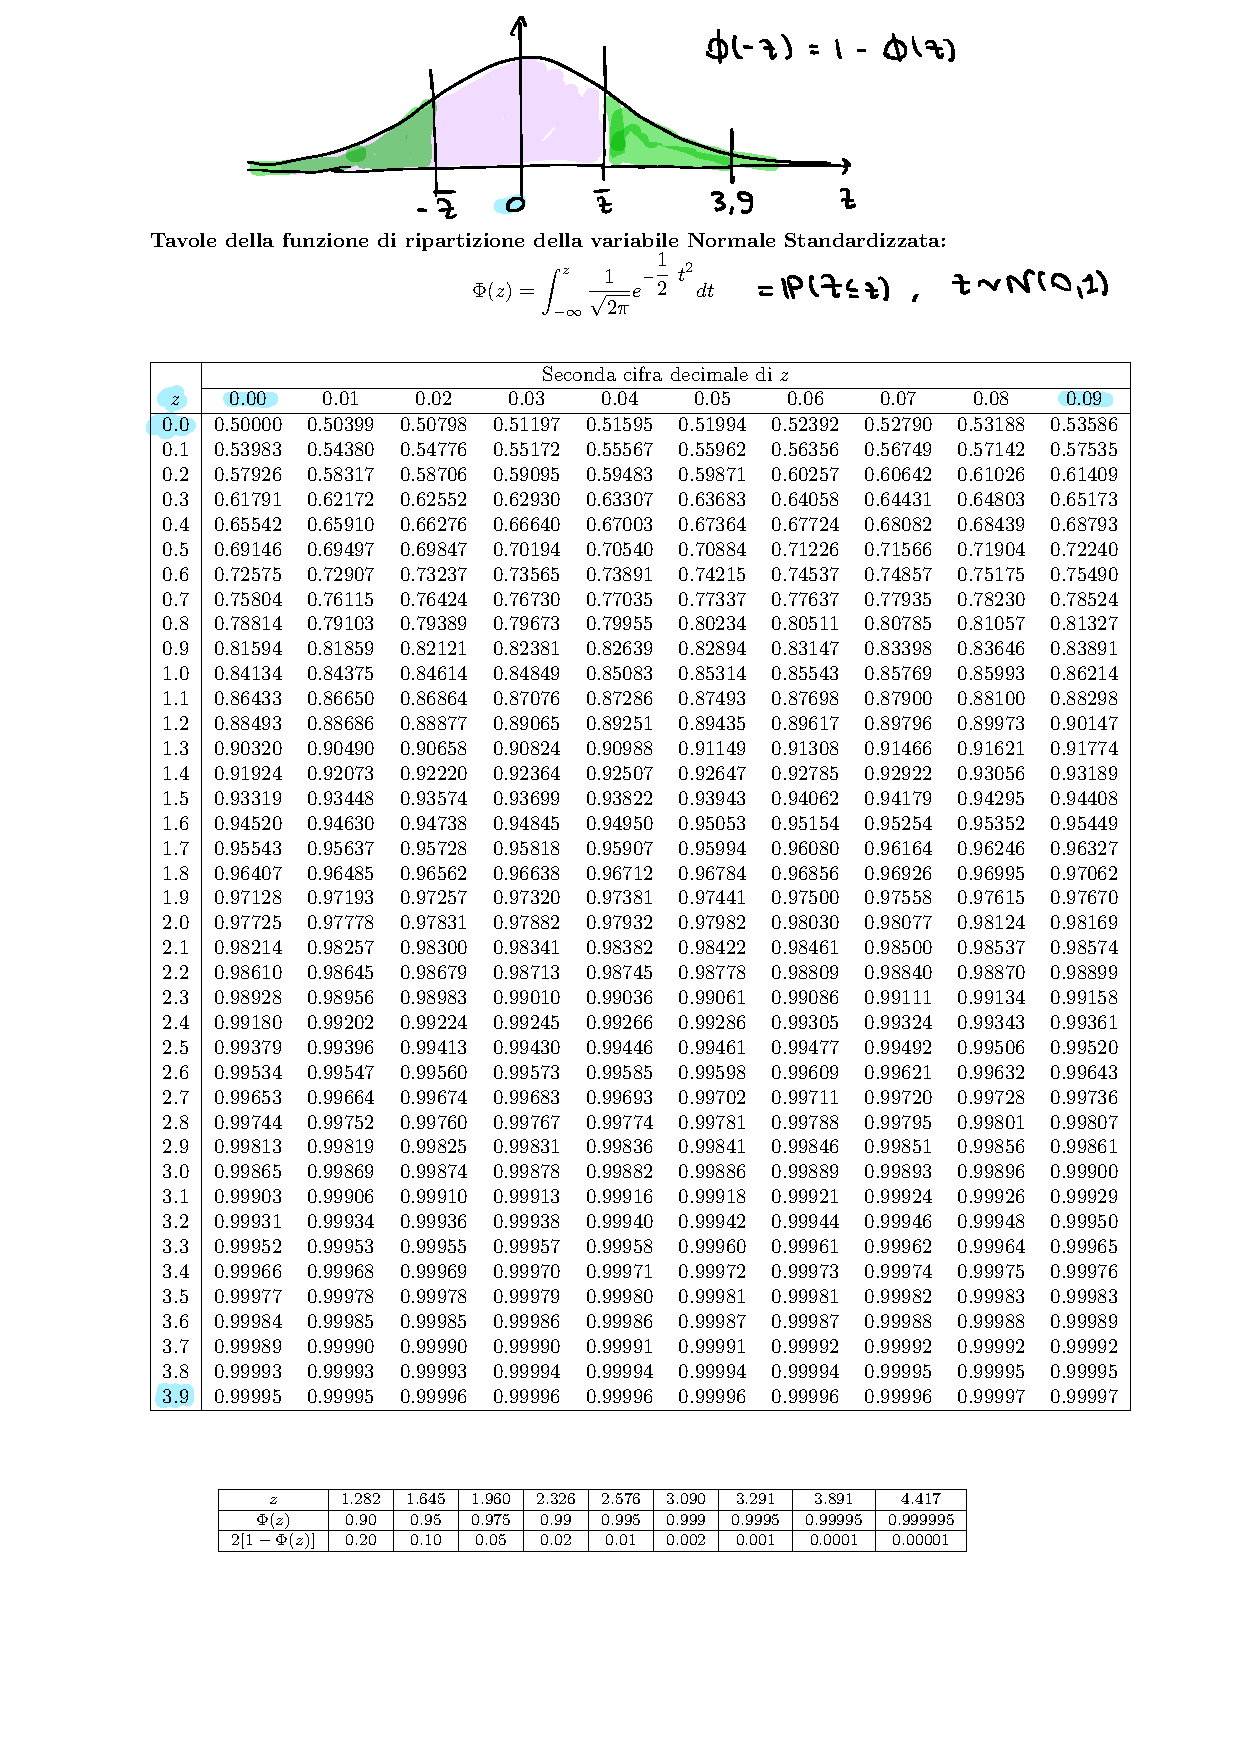
\includepdf[pages=-,scale=0.9]{tavola_normale.pdf}

\end{document}
